\subsubsection{Block-size-calculation}

Understanding how Bitcoin block size is calculated post-Taproot upgrade is crucial.

\paragraph*{block size}

The block size calculation is depicted in the following illustration:

\begin{figure}[ht] 
    \centering  
    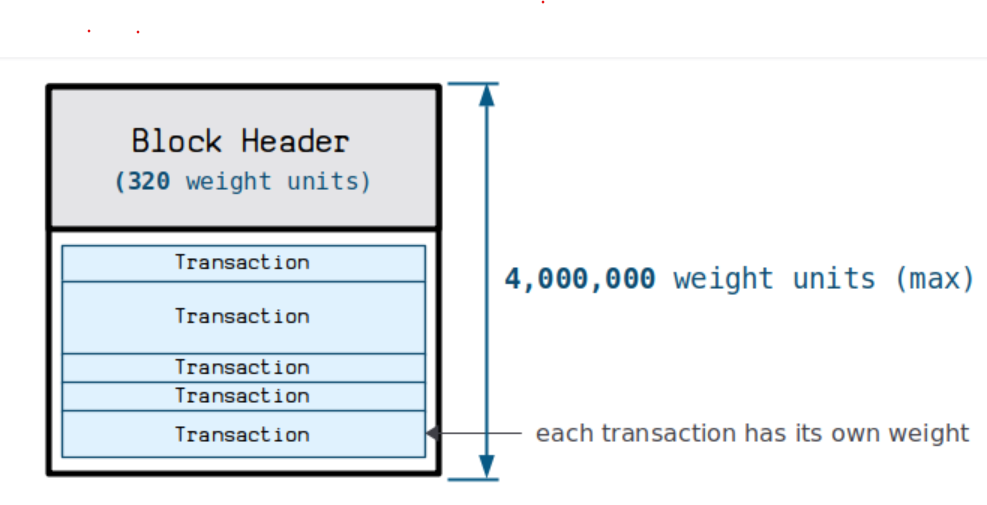
\includegraphics[width=0.85\columnwidth]{images/block-size.png} 
    \caption{Block size}
    \label{fig:block-size}
\end{figure}

\paragraph*{transaction size}

The transaction size calculation is illustrated below:

\begin{figure}[ht] 
    \centering  
    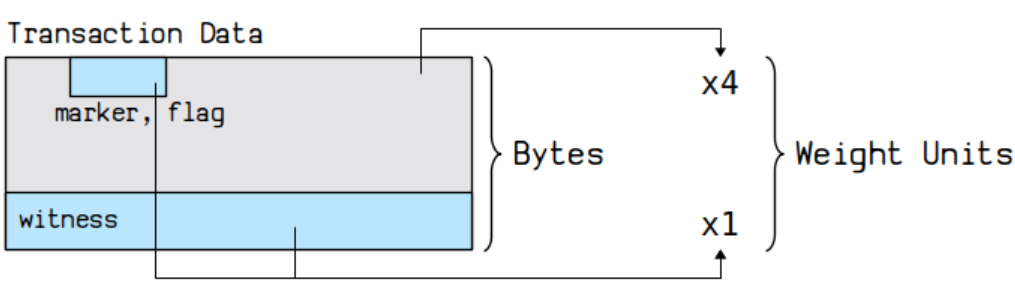
\includegraphics[width=0.85\columnwidth]{images/transaction-size.png} 
    \caption{Transaction size}
    \label{fig:transaction-size}
\end{figure}

For more detailed information, refer to source in \cite{website:transaction-size}

\paragraph*{script chunk limitation}

Based on the deign of BitVM2 \cite{website:BitVM2}, we hope each script chunk could be packed into one block as a transaction.
So, the transaction size could not exceed 4,000,000 - 320 = 3,999,680 weight units \cite{website:transaction-size}.

The disputed transaction is a 1 input and 2 outputs, the average size of non-witness data in this kind of transaction is around 464 weight units.
So for the witness size, the limitation is 3,999,680 - 464 = 3,999,216 weight units.

As showed in BitVM2 \cite{website:BitVM2}, the disputed transaction needs to the signature of Committee, and the sign type is
SIGNHASH\_SINGLE. Let's assume that the number of Committee is 7 and the size of each schnorr signature is 65 bytes (64 bytes for SIGNHASH\_ALL)

So the limitation will be 3,999,216 - 7 * 75 - 8(stack item size) = 3,998,683 weight units.

\begin{figure}[ht] 
    \centering  
    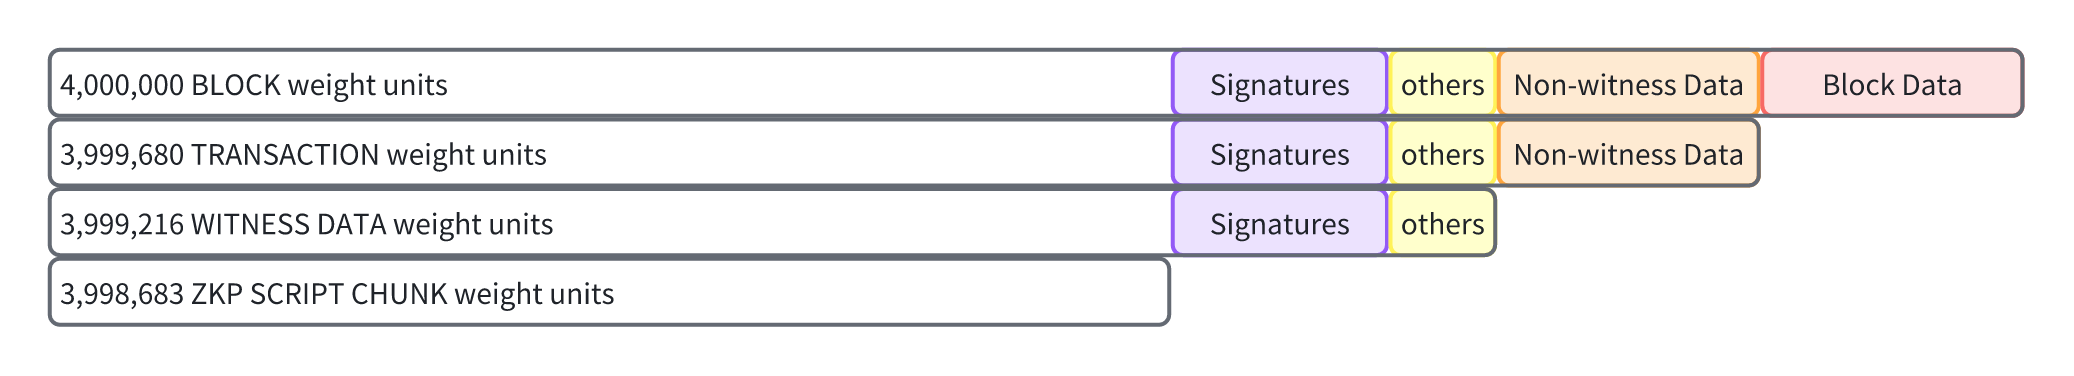
\includegraphics[width=0.85\columnwidth]{images/ZKP-script-chunk-limitation.png} 
    \caption{ZKP script chunk limitation}
    \label{fig:ZKP-script-chunk-limitation}
\end{figure}
